\documentclass{report}
\usepackage{color}
\usepackage[utf8x]{inputenc}
\usepackage[T1]{fontenc}      % caractères français
\usepackage{geometry}         % marges
\usepackage[francais]{babel}  % langue
\usepackage{graphicx} 
\usepackage{wrapfig}
\usepackage{listingsutf8}
\usepackage[final]{pdfpages} 
\usepackage{float}
\usepackage{listings}
\usepackage{amsmath}
\usepackage{enumitem}     % images
\usepackage{verbatim}         % texte préformaté
\title{\LARGE Implémentation d'un outil de veille concurrentielle concernant des articles de loisirs sportifs}      % renseigne le titre
\author{Clément BALESTRAT - Nicolas KERMARC - Yann PRAVOSSOUDOVITCH}
          
\pagestyle{headings}          % affiche un rappel discret (en haut à gauche)
                         % de la partie dans laquel on se situe
                         
\makeatletter
\def\thetitle{\@title}
\def\theauthor{\large\@author}
\def\thedate{\@date}
\makeatother
\definecolor{light-gray}{gray}{0.95}
\lstset{backgroundcolor=\color{light-gray}, inputencoding=utf8/latin1}
\begin{document}
\begin{titlepage}


\includegraphics[scale=0.1]{logo.jpg} 

\centering
\vfill
{\Huge\bfseries \thetitle}
\vskip 1cm
{\Large \theauthor}
\hspace{10.5cm}
\vskip 0.25cm
\Large Rapport de synthèse du Projet Industriel de Fin d'Etudes\\
\Large Département Informatique et Gestion
\vskip 0.25cm
\Large 25 janvier 2013
\vskip 0.5cm
\vfill
\large Tuteur: Anne-Laure De Lauzun
\hspace{2cm}
\large Demandeur: Sébastien BERNIS
\end{titlepage}



\renewcommand{\contentsname}{Sommaire}
 


\tableofcontents

\chapter{Introduction}

\paragraph{}

Dans le cadre de nos études, un Projet Industriel de Fin d'Etudes (PIFE) est à réaliser par groupe d'étudiants. Ce projet, étalé sur une période de deux mois a pour but de faire travailler les étudiants sur un sujet pour une entreprise, tout en restant dans le cadre des études. Ce rapport a donc pour but de faire une synthèse de notre travail durant cette période.

\paragraph{}

Dans une première partie nous verrons donc le contexte de ce projet, avec une brève présentation du demandeur ainsi qu'une description de la demande initiale. \\Puis, dans une seconde partie, notre démarche ainsi que notre organisation utilisées pour mener à bien notre travail seront décrites. \\La partie suivante traitera notre travail effectué. Les résultats intermédiaires et finaux, mais aussi les problèmes techniques seront ici détaillés. \\Enfin une conclusion viendra clôturer ce rapport, avec un bref récapitulatif sur les tenants et les aboutissants de ce projet, mais aussi ce que ce dernier a apporté au groupe et à l'entreprise.
\chapter{Le contexte}

\section{Sébastien BERNIS}

\paragraph{}

Nous avons choisi d'effectuer ce projet industriel pour la société \textit{BERNIS Informatique}, représentée par Sébastien Bernis.
Actuellement employé chez \textit{La Palanquée}, magasin de produits concernant la plongée sous marine à Palavas-les-Flots, Sébastien Bernis a notamment pour tâche la gestion du site internet de l'entreprise, proposant une plateforme de e-commerce.
\newline
Ayant l'habitude de surveiller les articles chez les concurrents, ce dernier s'est rendu compte que les sites de comparaison de prix n'étaient pas des plus justes, car ils auraient la fâcheuse tendance à baser leur affichage en fonction des sociétés qui payent le plus, et non en fonction des prix réels. Il a donc eu pour idée la création d'une véritable plateforme de comparaison de prix en temps réel. Ce service serait proposé uniquement aux professionnels, qui, à n'importe quel moment de la journée pourraient consulter les prix de leurs concurrents directs.



\section{Notre mission}

\paragraph{}

Nous avons donc eu pour mission le développement de ce module de comparaison de prix. L'utilisateur se connectera sur le site et accèdera directement à une page principale avec d'un côté ses prix à lui, et d'un autre les prix de ses concurrents. Il sera donc important de mettre en valeur les prix étant moins chers ailleurs, afin que ce dernier puisse s'en apercevoir rapidement.

\paragraph{}

Deux points semble être ici relativement importants: la bonne récupération des prix et l'afficage de ces derniers en temps réel. 
\\Un identifiant unique pour chaque article n'étant certainement pas présent à tous les moments, il sera donc important d'essayer de faire correspondre au mieux les désignations et modèles de ces derniers. Il arrive que les prix puissent varier plusieurs fois dans la journée. Il est donc primordial d'afficher les bons prix à l'utilisateur. Notre algorithme devra par conséquent être des plus efficace, afin de proposer une mise à jour des tarifs très rapidement.\\
Il est bien évidemment nécessaire de traiter uniquement les articles que l'utilisateur possède. Ce dernier n'aura pas besoin de consulter des prix pour des produits qu'il ne vend pas.
\\
Pour l'instant notre projet a été limité à quelques sites d'articles de plongée comme \textit{scubastore.com}, \textit{palanquee.com}, \textit{bubble-diving.com}, \textit{vieuxplongeur.com} et \textit{scubaland.com}.   

\paragraph{}

Il faut bien comprendre que mis à part ces détails, aucune indication supplémentaire nous a été donnée. C'est d'ailleurs pour ça que ce projet nous a séduit au départ. En effet, il nous a donné la possibilité de partir de rien pour espérer arriver à un rendu exploitable. Un long travail de conception, d'implémentation et de déploiement nous attendait. Bien évidemment pour chaque choix conceptuel nous avons pu en parler directement avec M. Bernis qui s'est porté volontaire, dès le départ, à nous rencontrer chaque semaine afin de faire le point sur nos avancements. Nous avons eu cependant une totale liberté de mouvement vis à vis des choix technologiques.

\paragraph{}
Notre premier travail a donc été la rédaction de la lettre de mission, afin de clarifier tous les points au sujet de ce que voulait le demandeur.
De ce fait, un listing récapitulatif des fonctions de l'application a été établi:

\begin{itemize}
\item Récupération des articles et des prix sur les sites précédemments cités à l'aide de scripts automatiques dits \textit{robots}.
\item Développement d'une interface utilisateur relativement basique, mais claire.
\item Gérer l'affichage des articles que vend l'utilisateur et y associer les prix des concurrents, tout en mettant en valeur ceux qui sont inférieurs.
\item Implémenter un système de mise à jour des prix et des articles afin que l'utilisateur puisse toujours avoir des données correctes.
\end{itemize}

\paragraph{}
C'est donc à partir de cette liste que nous avons pu démarrer notre travail.

\chapter{Organisation et démarche}

\section{Découpage des tâches et établissement des rôles}
Notre premier travail fût l'analyse des différentes tâches qui allaient composer ce projet. Nous avons pu très vite distinguer plusieurs axes de réflexion et de travail:

\begin{itemize}
\item L'étude de la structure des sites web concernés, afin de voir comment y récupérer les données.
\item La réflexion sur le stockage de ces données. Quel type de base de données ? Quelle(s) structure(s) ? Quel(s) modèle(s)
\item Le choix d'un rendu visuel. Avoir quelque chose de clair, ergonomique et esthétique qui puisse intéragir avec la base de données.
\end{itemize}

\paragraph{}
Nous avons donc pu, dans un premier temps, définir les rôles de chacun. Nicolas Kermarc serait responsable du rendu visuel (\textit{front-end}), Clément Balestrat de la collecte des données sur chacun des sites et Yann Pravossoudovitch responsable de la base de données. \\Pourquoi avoir effectué ce découpage par rôle ? \\Tout simplement parce que nous avons trouvé judicieux le choix de se spécialiser chacun dans un domaine bien précis du projet afin d'être le plus compétent possible, au lieu de "toucher à tout" ce qui au final aurait pu provoquer une perte de temps et un cafouillage général.\\
Ainsi, le travail de Clément serait complémentaire à celui de Yann puisque ce dernier aurait besoin de toutes ces données pour les stocker, et c'est ce stockage qui allait être utile à Nicolas pour pouvoir gérer l'interface utilisateur.\\
Pour ce qui est de la conception générale du projet, il est bien évident qu'un travail d'équipe a eu lieu afin de pouvoir réfléchir tous ensemble et se mettre d'accord sur une idée finale.

\section{La gestion de projet}

\paragraph{}

Ce projet nous a très vite paru lourd en matière de charge de travail. En effet, avec deux mois pour une conception, un développement et un déploiement, le tout accompagné d'une rédaction de rapport de synthèse et technique, il fallait trouver une organisation optimale dans le temps. Après avoir établi le nombre de jours/homme nécessaire au bon déroulement de ce projet, nous avons décidé d'utiliser un diagramme de Gantt afin d'avoir un planning à suivre.

\begin{figure}[H]
\begin{center}
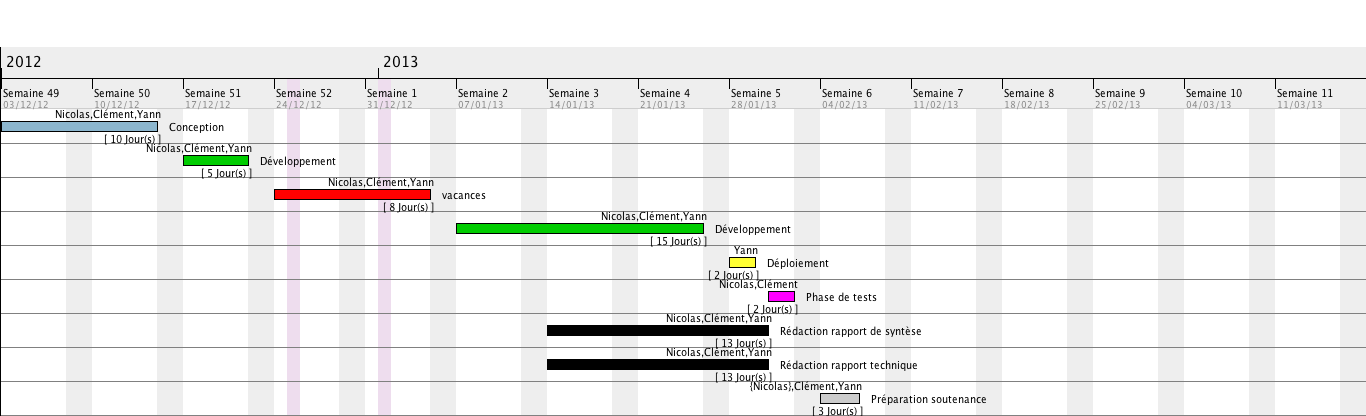
\includegraphics[scale=0.4, angle=90]{diagramme.png}
\caption{\textit{Diagramme de Gantt}}
\end{center}
\end{figure}

\paragraph{}
Comme on peut le voir sur la figure 3.1, les tâches suivantes ont été programmées dans le planning:
\begin{itemize}
\item Conception (10 jours)
\item Développement (20 jours)
\item Rédaction du rapport de synthèse et du rapport technique (13 jours)
\item Déploiement de l'application (2 jours)
\item Phase de tests (2 jours)
\item Préparation de la soutenance (3 jours)
\end{itemize}


\paragraph{}
Plusieurs tâches ont été placées en même temps, comme le développement et la rédaction des rapports. C'est tout simplement qu'un roulement a été plannifié. En effet, à partir du 14 janvier, deux auront pour tâche le développement pendant qu'un autre s'occupera du rapport. Ce roulement est journalier mais peut être allongé pour des raisons particulières (une partie à finir de rédiger pour la personne concernée par exemple). \\

Nous avons jugé que deux personnes étaient utiles pour la rédaction du rapport de synthèse (Clément et Nicolas), et trois personnes pour le rapport technique. Etant donné que chacun aura une mission technique relativement différente durant le projet, il nous a donc semblé normal que chacun détaille sa partie au mieux dans le rapport technique.\\

Pour finir, Yann sera chargé de la partie déploiement tandis que Clément et Nicolas s'occuperont des tests finaux. Un créneau de trois jours à également été réservé afin de pouvoir se préparer pour la soutenance du projet.

\section{Nos outils}
Les choix technologiques ont été établis très rapidement: 
\begin{itemize}
\item PHP pour la partie récupération de données sur les sites de plongée
\item MongoDB pour la gestion de la base de données
\item Node.js pour le front-end
\end{itemize}

\paragraph{}
Pourquoi ces technologies et pas d'autres ? Le PHP est un langage web énormément utilisé et est réputé pour sa rapidité de traitement. Ayant une grosse communauté de développeurs, il possède tout un arsenal de librairies qui va nous servir à récolter très facilement les données sur les sites. \\MongoDB est un Système de Gestion de Base de Données (SGBD) scalable, à hautes performances et open source. Nous avions déjà eu l'occasion de l'utiliser lors du précédent projet industriel chez \textit{Deegr.com} et sa facilité d'utilisation nous avait charmés.\\Enfin, Node.js car il permet de faire du JavaScript côté serveur, et est réputé pour ses bonnes performances.\\
Une description plus détaillée sur ces technologies est présente dans le rapport technique.

\paragraph{}
En ce qui concerne les outils de travail collaboratif, nous avons utilisé Github, qui est un logiciel de versions décentralisées. Il permet à un groupe de développeurs de travailler sur un même projet sans avoir à s'envoyer les sources à chaque fois qu'elles ont été mises à jour. En effet, un simple \textit{push} permet à une membre de l'équipe de mettre à jour ses changements sur le serveur Git, et \textit{pull} pour récupérer la dernière version du projet sur son poste.\\
Cet outil est indispensable pour le bon déroulement d'un projet en équipe.

\begin{figure}[H]
\begin{center}

\includegraphics[scale=0.4]{git.png}
\caption{\textit{Github}}
\end{center}
\end{figure}

\paragraph{}
Enfin, M. Bernis a eu l'idée de nous louer un serveur dédié chez OVH afin de pouvoir héberger notre projet, mais aussi dans le but de gagner en performance lors de l'exécution des robots ou de l'algorithme de matching, cette dernière pouvant être fastidieuse et gourmande en ressources, poussant souvent nos Macbook Pro dans leurs derniers retranchements.

\begin{figure}[H]
\begin{center}

\includegraphics[scale=1.2]{ovh.jpg}
\caption{\textit{OVH}}
\end{center}
\end{figure}

\chapter{La conception}

\paragraph{}
Ce chapitre est essentiel car il va permettre au lecteur de comprendre notre façon de penser. N'ayant pas vraiment de pistes au départ, notre travail s'est fait à tâtons dans les débuts. 
\section{Les modèles}

\paragraph{}

Ce projet est principalement basé sur les données que nos parseurs\footnote{Synonyme de robot, crawler, spider.} vont récupérer. Par conséquent il fut important de réfléchir sur la structure de nos modèles en BD\footnote{Acronyme de Base de Données}. A première vue, le plus important sur la page d'un article est son libellé et son prix. En effet, comme précisé plus haut, il n'existe pas de numéro unique pour un article, comme l'ISBN pour un livre par exemple. Nous avons pensé à la référence du modèle, mais cette dernière est absente sur certain sites, et M. Bernis nous a expliqué que certain magasin se créent les leurs donc il se peut qu'il n'y ait aucun rapport avec celui donné par le constructeur.\\
Notre comparaison serait donc basée sur le libellé de l'article ainsi que le prix. En effet, le fait de constater que le prix d'un article que l'on souhaite comparer avec le notre se trouve à peu près dans la même fourchette de tarif nous a semblé être une idée intéressante.

\paragraph{}
Parcourir tous les sites pour "aspirer" le libellé et le prix des articles va prendre énormément de temps. Il faudra donc garder une trace de l'URL de l'article afin de pouvoir réutiliser cette dernière si besoin. Pour une mise à jour des prix par exemple: on se rend à l'article concerné dans la BD, on récupère son URL et on va chercher le nouveau prix.
Notre modèle \textit{article} possèdera donc un attribut \textit{Url}.

\newpage
\paragraph{}
Pour l'instant notre collection\footnote{Equivalent de "table" en SQL, chez MongoDB.} \textit{articles} se résume à ceci:


\begin{lstlisting}
Articles: (_id, url, _site, name, prices)

Avec:

_id: ID de l'article
url: l'url de l'article
_site: l'ID du site sur lequel est pris l'article
prices: le prix actuel de l'article
\end{lstlisting}

\paragraph{}
L'attribut \textit{\_sites} faisant référence à l'ID du site sur lequel est pris l'article, il est donc bien évident qu'une collection \textit{Sites} sera présente.
A première vue le modèle basique serait:

\begin{lstlisting}
Sites: (_id, url)

Avec:

_id: ID du site
url: l'url du site
\end{lstlisting}

\paragraph{}
Théoriquement cette conception pourrait nous permettre d'inscrire tous les sites concernés dans une collection, et de récupérer tous les articles de ces sites dans une autre.
Car c'est sans aucun doute le premier "gros travail" de ce projet: récupérer le plus d'articles possible sur ces plateformes e-commerce.

\newpage
\section{Idées supplémentaires}

\paragraph{}
Durant la phase de réflexion concernant la conception, plusieurs idées nous sont venues.\\
Tout d'abord, la possibilité pour l'utilisateur de consulter la courbe de variation des prix sur un article donné. Beaucoup de sites proposent ce service, et il est vrai qu'il peut s'avérer utile dans certains cas. Pour se faire, il faudrait très légèrement modifier la collection \textit{Articles} afin de pouvoir associer une date à un prix. L'attribut \textit{Prices} deviendrait donc un tableau d'objets avec à l'intérieur un prix auquel on associer une date. Ainsi, via l'aide d'un framework en Javascript pour les graphes (Flotr), on va pouvoir récupérer ce tableau et tracer une courbe d'évolution des prix.

\begin{figure}[H]
\begin{center}
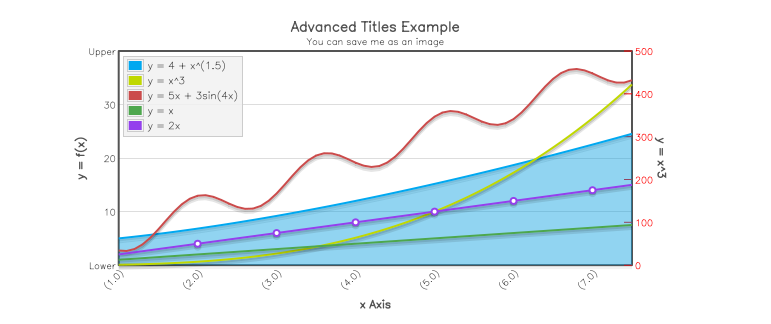
\includegraphics[scale=0.6]{flotr.png}
\caption{\textit{Un exemple de possiblité de graphe avec le framework Flotr}}
\end{center}
\end{figure}


\paragraph{}
Une autre idée est celle des catégories. Pour chaque article récupéré, essayer de prendre sa catégorie nous permettrait de filtrer les affichages, les recherches...etc. Un seul problème: à première vue, les catégories ne sont pas les mêmes selon les sites, donc il y aurait tout un travail de recherche de correspondance et de recoupement de catégories derrière. Ceci dit nous allons voir plus tard que c'est grâce à ces catégories que nous avons pu résoudre une grosse partie de nos problèmes.

\newpage
\paragraph{}
Une mise à jour des modèles \textit{Artciles} et \textit{Sites} est donc nécessaire:

\begin{lstlisting}
Articles: (_id, url, _site, name, prices[price, date], category)
Sites: (_id, url, name_cat, name_gen)

Avec:

prices, le tableau qui associe un prix avec une date
category, la categorie de l'article
name_cat le veritable nom de la categorie (specifique au site)
name_gen le nom generique trouve pour recouper les categories entre elles 
\end{lstlisting}

\paragraph{}
Une dernière amélioration possible serait de pouvoir exporter le tableau des prix des articles au format XLS, afin de pouvoir travailler dessus sur Excel, ou tout simplement l'imprimer. Il existe énormément de librairies pour traiter ce genre de cas en PHP, ce qui rend donc cette tâche très largement faisable.

\section{Le matching}

\paragraph{}
C'est ici que commence une partie également très intéressante pour ce projet, vu qu'elle représente la principale fonctionnalité. En effet, la recherche de correspondance ou \textit{matching}, est un élément primordial dans l'élaboration d'un outil de comparaison; elle va nous permettre d'associer les différents articles entre les sites afin de pouvoir en comparer les prix.\\

\begin{figure}[H]
\begin{center}
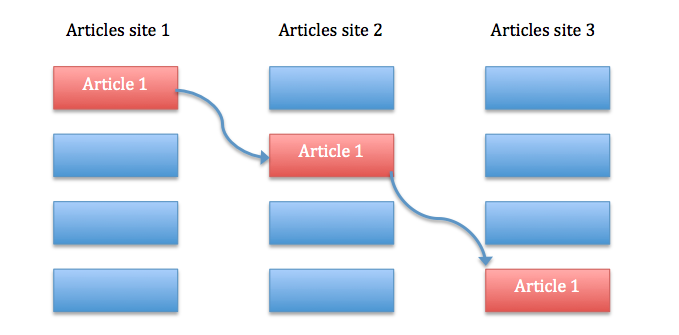
\includegraphics[scale=0.6]{articles.png}
\caption{\textit{Recherche d'une correspondance entre les articles de plusieurs sites}}
\end{center}
\end{figure}

\paragraph{}
On part donc d'un site référent, c'est à dire que l'on doit simuler le fait qu'un client veuille comparer les prix des articles de son site. Ici, on ne pourra bien évidemment choisir qu'entre les cinq sites du projet. Par exemple si on choisit \textit{palanquee.com} comme site référent, l'algorithme de matching va récupérer les articles de ce site, et chercher des correspondances avec les quatres autres. Ainsi uniquement les articles de La Palanquée vont être comparés.\\
Comment gérer l'inscription en base de données d'une correspondance ? C'est très simple, il suffira d'ajouter un attribut à la collection \textit{articles} nommé par exemple \textit{match} qui correspondra à un tableau d'IDs des articles correspondants. Un par site donc étant donné que l'on part sur la base d'un matching très précis\footnote{Nous verrons plus tard que justement, ce choix a posé problème}.\\
On a donc une fois de plus, une légère mise à jour de la collection \textit{articles}: 

\begin{lstlisting}
Articles:(_id, url, _site, name, prices[price, date], category, match[])

Avec:

match, un tableau d'IDs d'articles. Quatre cases dans ce tableau, 
pour les quatre articles trouves parmis les quatre autres sites

\end{lstlisting}

\paragraph{}
Ainsi une fois les correspondances trouvées et ajoutées dans ce tableau \textit{match}, il suffira juste de les récupérer afin de pouvoir travailler dessus en front-end\footnote{Partie visuelle du développement, s'oppose à \textit{back-end}}.


\section{Problèmes rencontrés}

\paragraph{}
Malheureusement tout ne s'est pas passé comme nous le voulions. En effet, après une analyse un peu plus précises des sites concernés, nous nous sommes rendus compte qu'un matching très précis allait être très difficile, voir impossible à réaliser. En effet n'ayant pas d'identifiant spécifique à un article, le seul moyen est la recherche de correpondance par libellés. Mais après avoir effectué plusieurs comparaisons entre ces derniers, nous en avons conclu qu'il y avait bien trop de différences pour pouvoir valider d'office une correpondance potentielle parmis les autres.\\
Un exemple de cinq libellés, correpondant au même article, sur les cinq sites.

\begin{lstlisting}
"Montre ordinateurs D6i Metal SUUNTO"
"Ordinateur D6i bracelet metal + interface incluse"
"Suunto D6i Elastomer White + Free Transmitter"
"Montre D6i Suunto bracelet acier avec Interface USB - Suunto"
"MONTRE D6I ALL BLACK - SUUNTO Aqualung"
\end{lstlisting}

\paragraph{}
Cet article, la montre D6i Suunto, pose problème. En effet, on peut voir chaque libellé est différent. L'ordre des mots n'est pas le même, des offres peuvent apparaître chez certains et pas chez d'autres...etc. Rien que rechercher un article directement sur les sites concernés (via leurs moteurs de recherche) peut s'avérer laborieux tellement les titres peuvent être différents. Ainsi même en possession du meilleur algorithme, nous ne pourrons jamais être sûrs que le bon article sera choisi.

\begin{figure}[H]
\begin{center}
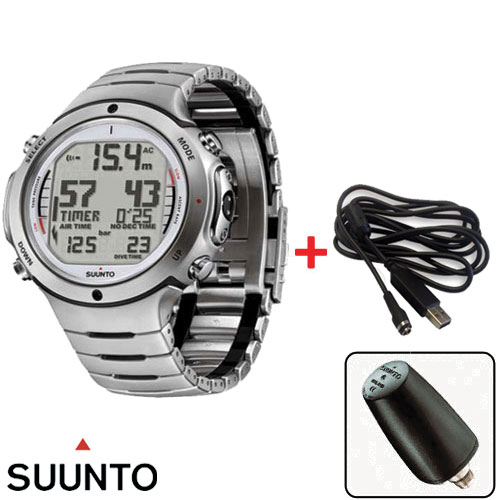
\includegraphics[scale=0.6]{montre.jpg}
\caption{\textit{Un exemple d'article: la montre D6i métal Suunto}}
\end{center}
\end{figure}


\paragraph{}
Autre problème: celui de récupérer tous les articles de tous les sites. La véritable technique serait de partir de la page d'accueil, et d'y récupérer tous les liens hypertexte, pour les analyser par la suite de la même façon que sur la page d'accueil et d'essayer de repérer lorsque l'un de ces liens pointe vers une page article. Un travail récursif donc, qui serait énormément laborieux à développer, voir même impossible en si peu de temps. En effet, un site de e-commerce possède des dizaines de milliers de liens, l'algorithme pourrait donc se perdre très facilement, ou dans le cas où ce dernier serait fonctionnel, mettrait des heures voir des jours à tout récupérer. Nos macbooks ne peuvent en aucun cas assurer le balayage de cinq sites de cette façon. Une saturation de la mémoire arriverait vite.

\paragraph{}
Le dernier obstacle est lié au fait que les catégories des sites peuvent être différentes. Il n'y a pas forcément les mêmes, ce qui pose donc problème pour toutes les réunir. Et bien évidemment, s'il manque des catégories, tous les articles ne pourront alors pas être récupérés.


\section{Orientation vers une nouvelle solution}

\paragraph{}
Tous les problèmes précédemment cités sont donc l'objet d'une nouvelle réflexion à propos de la création de cet outil de comparaison de prix. Une mise au point avec M. Bernis était donc nécessaire, afin de trouver un terrain d'entente à propos des fonctionnalités attendues.\\
Ce dernier a été très compréhensif et nous a donc aidé à trouver des solutions.

\paragraph{}
Au sujet du matching, nous avons eu l'idée de proposer une liste d'articles potentiellement identiques au produit référent à l'utilisateur, et c'est ce dernier qui devra les valider manuellement. Un repérage visuel donc, en fonction du libellé, mais qui peut être amélioré à l'aide de l'image des articles. Ainsi si l'image ou le libellé lui semble correspondre, il l'indiquera et ce choix sera sauvegardé en BD.\\
Une légère modification de la collection \textit{articles} est donc obligatoire.

\begin{lstlisting}
Articles: (_id, url, _site, name, prices[price, date], category, img)

Avec:

img, l'adresse de l'image de l'article

\end{lstlisting}

\paragraph{}
Ce changement va donc nous permettre de stocker l'url de l'image de l'article récupéré, et ainsi l'image pourra être affichée en visuel dans la liste des propositions de correspondances.

\paragraph{}
Ensuite est venue l'évocation du problème de récupération de tous les articles sur les sites. Quelles méthode de parsing utiliser ? Comment gérer les différentes catégories ?\\
Ceci s'est également réglé assez facilement: au lieu de partir de la page d'accueil et de récupérer tous les liens, nous nous sommes mis d'accord sur le fait de partir directement des pages de catégories. Ces dernières ont des adresses bien spéciales, et contiennent un listing des articles qui en font partie.

\begin{figure}[H]
\begin{center}
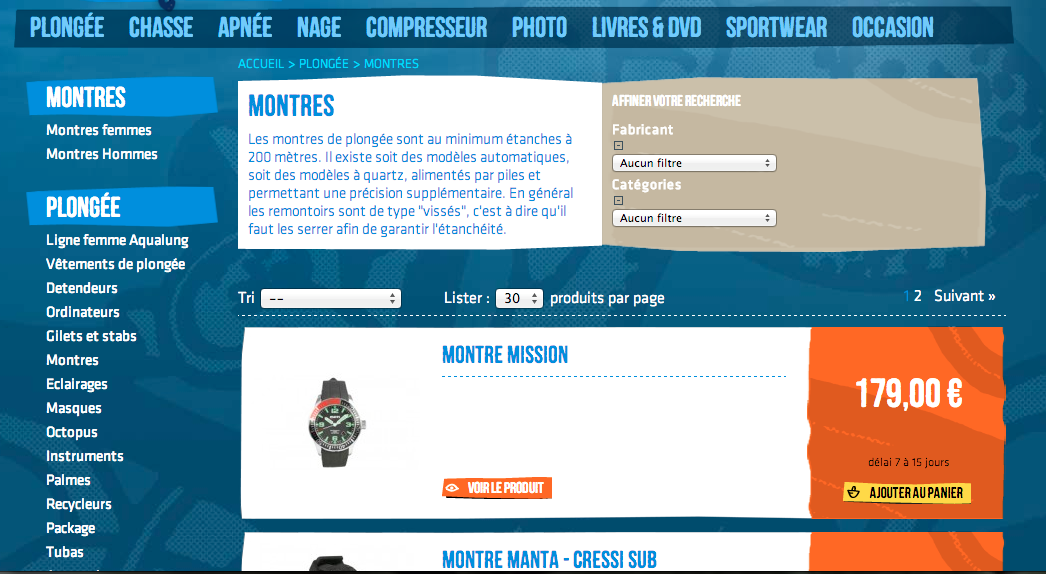
\includegraphics[scale=0.4]{vp.png}
\caption{\textit{Un exemple de la liste d'articles de la catégorie "ordinateurs" du vieuxplongeur.com}}
\end{center}
\end{figure}

\paragraph{}
Avec cette méthode, certes plus ciblée et un peu moins automatique (les adresses des différentes catégories doivent être ajoutées manuellement), nous avons directement accès à des pages articles.\\
La correspondance entre les différentes catégories sera aussi un travail de recherche avant tout. Nous essayerons de trouver le plus de points communs entre ces dernières et nous laisseront de côté celles où qui sont spécifiques à un seul site. Ainsi, nous avons réussi à faire correspondre 13 catégories:

\begin{itemize}
\item Ordinateurs
\item Palmes-masques-tubas
\item Montres
\item Sacs
\item Bouteilles
\item Combinaisons
\item Eclairages
\item Arbalètes
\item Lestage
\item Chaussons
\item Gants
\item Gilets
\item Bouées
\end{itemize}

\paragraph{}
Avec cette méthode, nous ne pouvons nier le fait que nous perdons un certain nombre d'articles par sites, mais cette dernière nous permettra de nous constituer une base de données d'articles quand même très impressionnante (environ 10 000) et d'avoir quelque chose de fonctionnel à la fin.\\
De plus nous proposerons la possibilité pour l'utilisateur d'ajouter un article manuellement via la copie de l'url directement dans une boîte de dialogue. Par conséquent, lorsqu'un article sera manquant, il sera toujours possible de l'ajouter manuellement. L'ajout manuel va également concerner le matching. Si la liste de recommendations d'articles est vide ou ne propose pas les bons produits, l'utilisateur pourra ajouter la bonne correspondance à la main, via l'adresse de l'article.


\section{Maquettes}

\paragraph{}
Afin de valider définitivement les fonctionnalités du site, nous avons réalisé des maquettes. Ces dernières ont ensuite été soumises à M. Bernis, qui nous a donné son accord pour le rendu final.

\begin{figure}[H]
\begin{center}
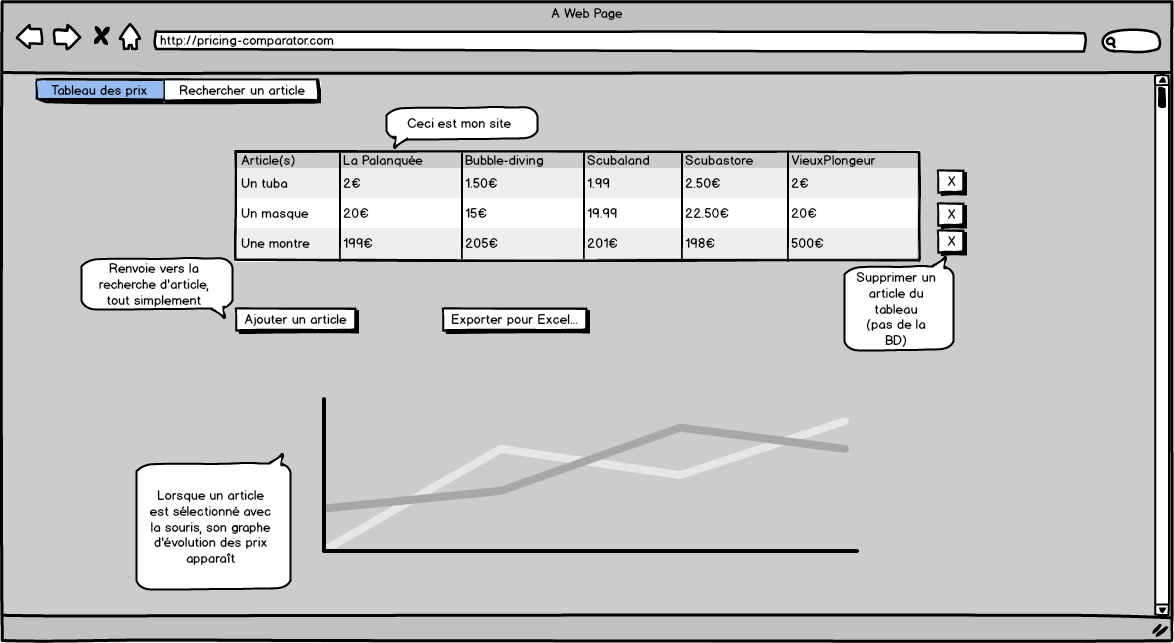
\includegraphics[scale=0.4]{home.png}
\caption{\textit{La page d'accueil}}
\end{center}
\end{figure}

\begin{figure}[H]
\begin{center}
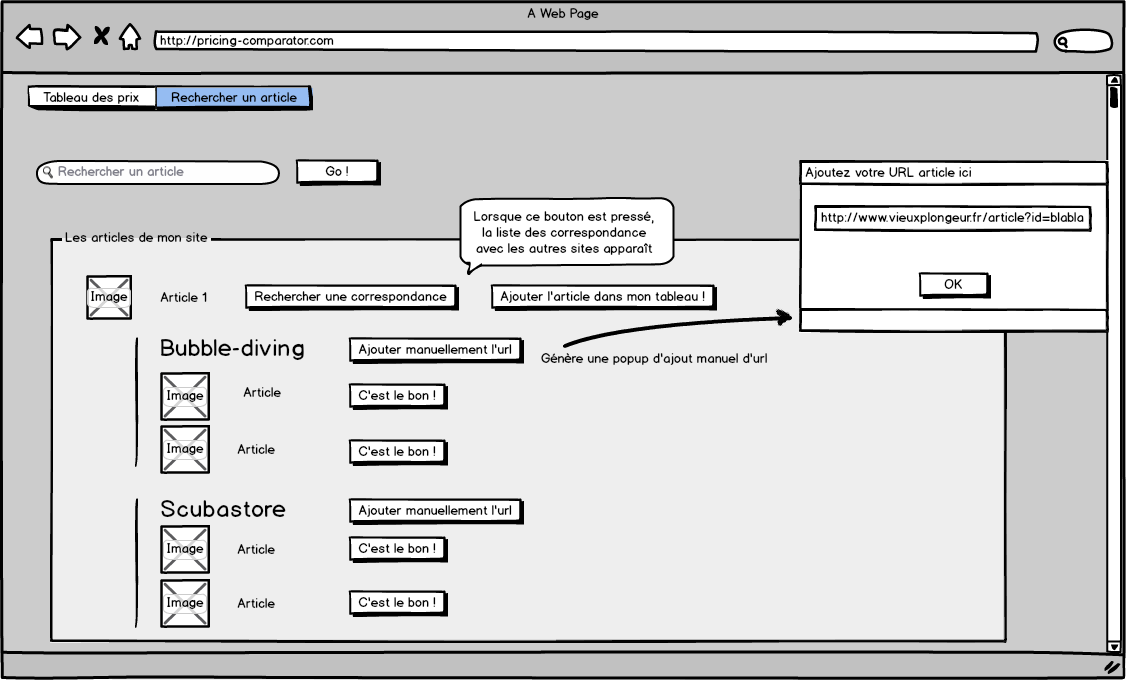
\includegraphics[scale=0.4]{search.png}
\caption{\textit{La page de recherche d'articles}}
\end{center}
\end{figure}


\paragraph{}
Ces maquettes ont été réalisées avec l'aide du logiciel \textit{Balsamiq Mockups}. Il propose toute une panoplie d'outils aussi bien pour les maquettes de sites web que pour les applications mobiles. Les plus grosses firmes l'utilisent pour leurs projets, comme Apple, Google, Skype, IBM...etc.

\paragraph{}
Nous avons essayé d'être les plus précis sur ces maquettes, jusqu'à annoter certaines fonctionnalités à l'aide de "bulles" pour être sûrs de bien se faire comprendre par le demandeur.\\
L'utilisateur aura donc la possibilité de "suivre" le prix de certain articles dans un tableau (avec possibilité de les retirer si besoin). Pour aller chercher ces articles, il se rendra sur la page de recherche. Un barre de recherche ainsi qu'un filtrage par catégorie sera possible. Une fois le bon article (de sa base de données donc) trouvé, une liste de correspondances provenant des autres sites apparaîtra. Il aura alors la possibilité de préciser quels sont les bons, ou alors de les ajouter directement manuellement via l'adresse des articles. 



\chapter{Le développement}

\paragraph{}
Afin d'être le plus clair possible dans ce rapport de synthèse, nous avons fait le choix de ne pas parler de nos méthodes de développement. En effet il est difficile d'expliquer cette partie sans utiliser un langage  que certains pourraient juger d'incompréhensible. Pour plus de précisions concernant ce sujet nous encourageons donc fortement le lecteur à se reporter au rapport technique, où tout sera indiqué en détail.\\
Cette partie sera donc utilisée pour montrer les résultats finaux de ce projet, et de voir comment se sont adaptés le design et les fonctionnalités présentes dans les maquettes en "vrai".


\section{Le résultat final}

\paragraph{}
Commençons tout d'abord par une série d'impressions écran de l'application.

\begin{figure}[H]
\begin{center}
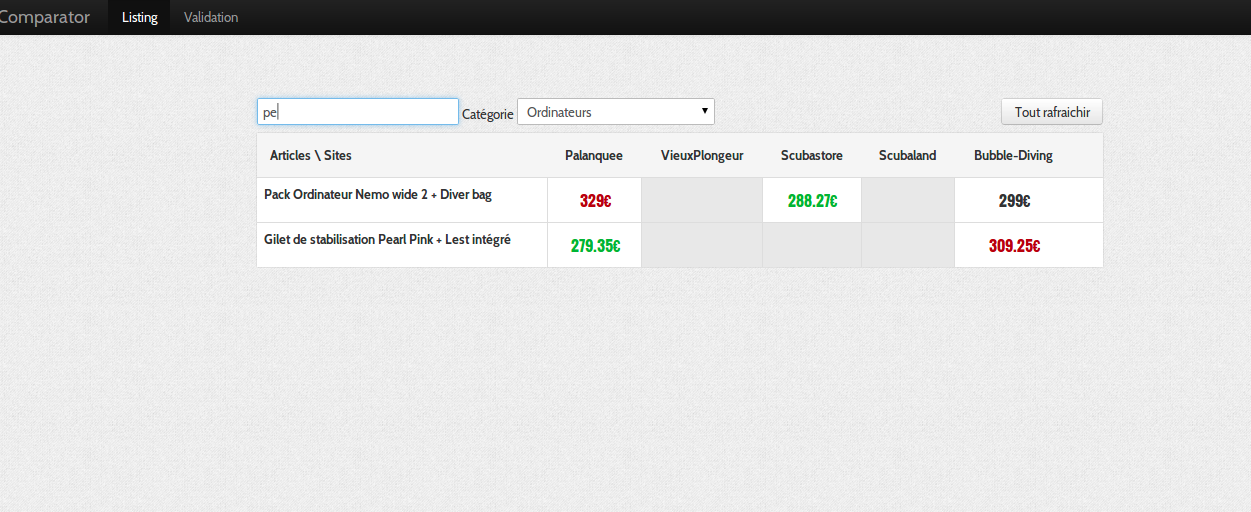
\includegraphics[scale=0.3]{1.png}
\caption{\textit{Le tableau de suivi des prix}}
\end{center}
\end{figure}

\begin{figure}[H]
\begin{center}
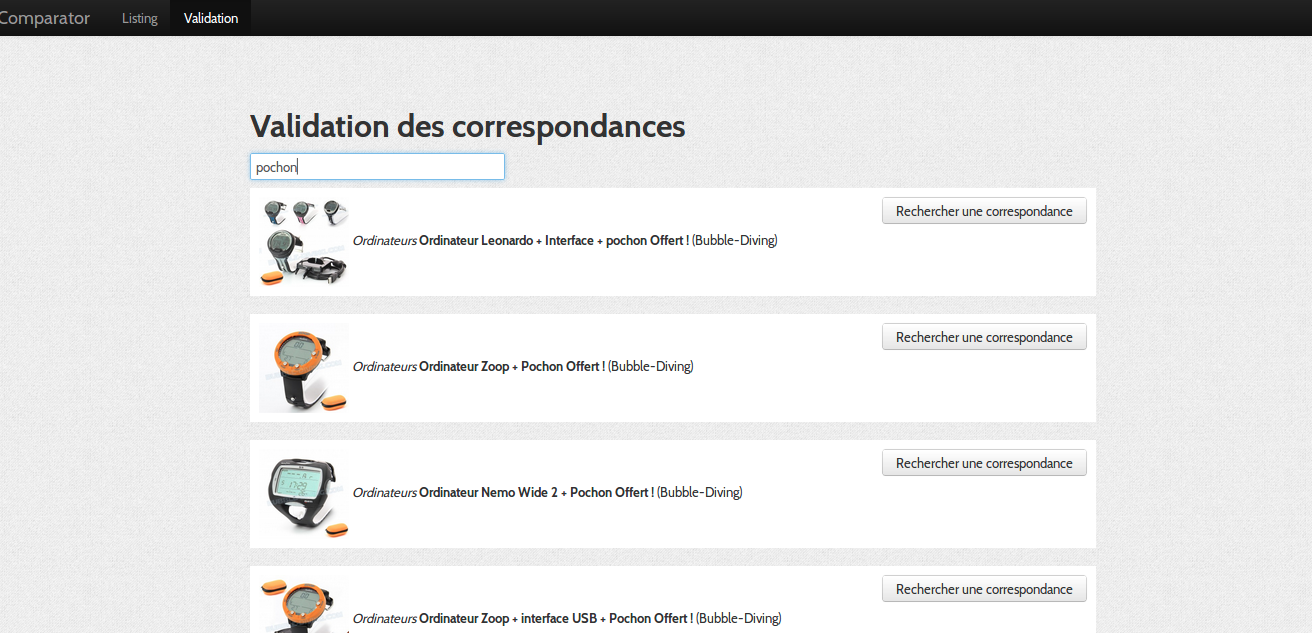
\includegraphics[scale=0.3]{2.png}
\caption{\textit{La page de recherche d'articles}}
\end{center}
\end{figure}

\begin{figure}[H]
\begin{center}
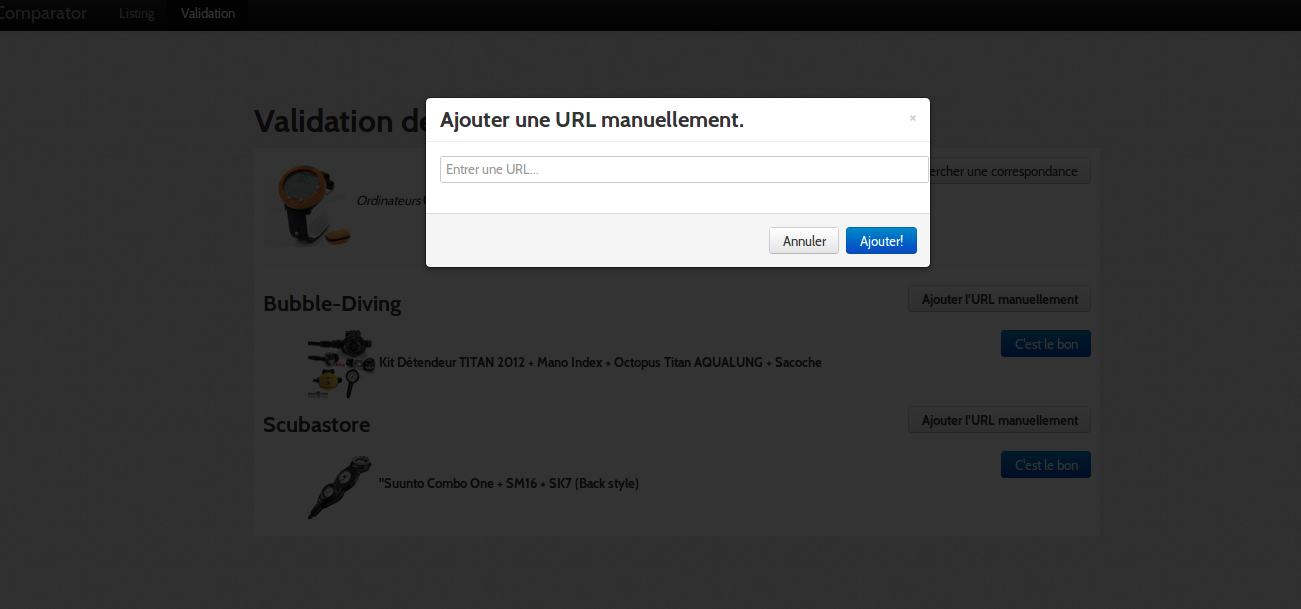
\includegraphics[scale=0.3]{3.png}
\caption{\textit{L'ajout manuel d'URL}}
\end{center}
\end{figure}


\begin{figure}[H]
\begin{center}
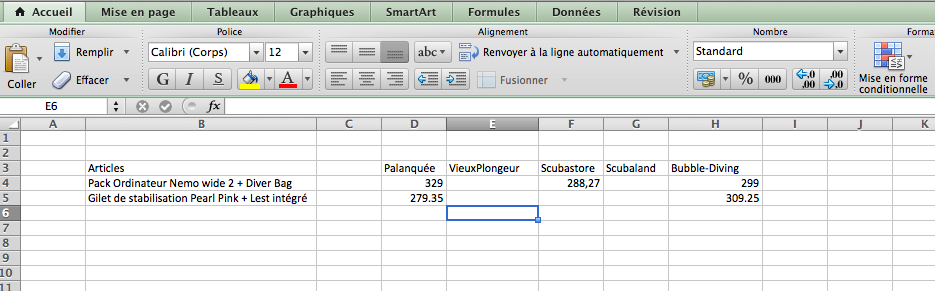
\includegraphics[scale=0.3]{4.png}
\caption{\textit{L'exportation au format XLS du tableau de suivi des prix}}
\end{center}
\end{figure}

\paragraph{}
Comme nous pouvons le voir, la charte graphique ainsi que les fonctionnalités ont été respectées. Le tableau met en valeur les prix moins chers (en vert) et ceux plus chers (en rouge). Il y a également une méthode de rafraîchissement manuelle, via le bouton \textit{Tout rafraîchir} qui a pour but de mettre à jour tous les prix présents dans le tableau. Il est en effet important d'avoir tout le temps les bons prix, dans le but de fournir un comparateur de prix de qualité.

\section{Problèmes techniques rencontrés}

\paragraph{}
Une fois les problèmes de conception résolus, nous n'avons pas véritablement fait face à de gros problèmes techniques. Les principaux étaient dûs en partie à une saturation de la mémoire de nos macbook lors du balayage de tous les sites. En effet, pour accéder à des valeurs comme le libellé ou le prix d'un article il nous a fallu repérer les bonnes balises dans le code source HTML des sites. Pour ce faire, des Data Object Model (DOM) ont été utilisés. Ces objets, réputés pour efficacité, le sont aussi pour leur "gourmandise" en matière de ressources. Quand trop de DOM sont créés et utilisés dans un script, la mémoire disponible baisse progressivement jusqu'à arriver à une saturation de celle ci.\\
Le code génère donc ce que l'on appelle une \textit{Segmentation fault (erreur de segmentation}, qui est une des plus connue (et parfois des plus redoutable) de la programmation.\\
Après quelques recherches nous avons vite trouvé d'où venait précisément le problème. Il fallait détruire chaque DOM à la fin de son utilisation. Ainsi, la mémoire est libérée progressivement, laissant place à la création et à l'utilisation d'autres DOM, sans générer d'erreur de mémoire. Des simples commandes commes \textit{unset} et \textit{clear} ont été mises à la disposition des développeurs pour gérer manuellement ce genre de problèmes.

\paragraph{}
Ces scripts étaient donc très longs à s'exécuter, du fait de la quantité d'articles à extaire, mais aussi parce qu'ils étaient plus ou moins tributaires de la qualité des serveurs des sites ciblés. Même avec une visite qualifiée de normale (via un navigateur internet) la plupart des sites ciblés par nos robots étaient lents. Ainsi, si 10 000 articles sont à récupérer sur ce genre de pages, cela prendra un temps considérable. Même si l'utilisation du serveur dédié mis à notre disposition nous a permis de gagner un peu de temps (les calculs se font beaucoup plus rapidement sur ce genre de machine que sur nos Macbooks), le remplissage de nos bases de données reste quelque chose de très long (plusieurs heures).


\chapter{Conclusion}

\paragraph{}
Ce projet a donc été bénéfique pour nous sur tous les plans. Nous avons pu participer à toutes les étapes de sa création, de la conception jusqu'au déploiement, nous permettant ainsi une véritable prise de décision concernant certain choix,  et résolutions de problèmes. Nous avons su recadrer le projet pour nous permettre d'avoir quelque chose de fonctionnel, sous contrôle et approbation du demandeur. Ce dernier a d'ailleurs toujours été présent pour nous aider et nous écouter, et nous l'en remercions pour ça.

\paragraph{}
Au niveau technique ce projet nous a permis d'aborder énormément de concept, comme les DOM en PHP, la manipulation d'énormément d'enregistrements en base de données, ainsi qu'une approche de technologies relativement récentes et à la mode en front-end, comme le framework Node.js.

\paragraph{}
Il est bien évident que beaucoup de travail reste à fournir sur ce projet, pour espérer d'en sortir un business plan vivable. Nous en avons réalisé les fondations ainsi que le coeur du fonctionnement, mais il serait intéressant que d'autres développeurs l'améliorent en implémentant par exemple une interface utilisateur, un système de facturation ainsi qu'en automatisant un peu plus certaines tâches, comme le parcours des sites à partir de la page d'accueil. L'ajout d'autres sites qui n'ont rien à voir avec la plongée pourrait être aussi un plus, afin d'étendre les domaines d'utilisation.

\paragraph{}
Pour finir, malgré l'énorme travail qu'a nécéssité ce projet, nous ne pouvons en tirer que des points positifs et sommes fiers de terminer nos études sur une mission de la sorte.\\





\end{document}
